\appendix

\section{Derivation of the recursion for $q_t$}
\label{Appendix:qt_derivation}

Recalling the definition $q_t \defeq s_{t-1} \cup \{a_{t-1},n_t\}$ and using the recursion \eqref{Equ:\modelname:s_t1}, we have
    \begin{align}
        q_{t+1}     &\overset{(a)}{=}  
                            s_t \cup \{a_t, n_{t+1} \}
                            \nn\\
                    &\overset{(b)}{=}
                            s_{t-1} \cup \{a_{t-1}, n_t, \mc{E}_{n_t}, \mc{N}_{n_t} \}
                            \cup \{ a_t, n_{t+1} \}
                            \nn\\
                    &\overset{(c)}{=}
                            q_t \cup \{ \mc{E}_{n_t}, \mc{N}_{n_t}, a_t, n_{t+1} \}
                            \nn
    \end{align}
where step (a) uses the definition of $q_{t+1}$, step (b) substitutes the recursion \eqref{Equ:\modelname:s_t1}, and step (c) uses the definition of $q_t$.


\section{Algorithm Implementation Details}
\label{Appendix:AlgDetails}

The detailed algorithm of \modelname~is described in Algorithm \ref{alg:reinforcewalk}. 
\begin{algorithm}[h]
	\begin{algorithmic}[1]
%	\SetKwInOut{Input}{Input}
	%\SetKwInOut{Output}{Output}
	\STATE {\bfseries Input: }{Graph $\mc{G}$; Initial node $n_S$; Query $q$;  Target node $n_{T}$; Maximum Path Length $T_{\text{max}}$; MCTS Search Number $E$;}
	%\Output{Target node $n_t$}
	\FOR{episode $e$ in $[1..E]$}
		\STATE Set current node $n_0 = n_S$; $q_{0} = f_{\theta_q}(q, 0, 0, n_0)$\;
		\FOR{$t=0\ldots T_{\text{max}}$}
%		\STATE Set Step $t = 1$\; 

		\STATE Lookup from dictionary to obtain $W(s_t, a)$ and $N(s_t, a)$ \;
		\STATE Select the action $a_{t}$ with the maximum PUCT value:
		\begin{align}
		a_t =
		\argmax_a \! \left\{ \! c \!\cdot\! \pi_{\theta}(a | s_t)^{\beta} \frac{\sqrt{\sum_{a'} N(s_t, a')}}{1 \!+\! N(s_t, a) } \!+\! \frac{W(s_t, a)} {N(s_t, a)}
		\!\right\} \nonumber
		\end{align}
		\STATE Update $q_{t+1} = f_{\theta_q}(q_t, h_{A, t}, h_{a_t, t}, n_{t+1})$\;
		\IF{$a_t$ is STOP}	
%		\STATE Go to Step 9 if $a_t$ is STOP; otherwise Step 13

		\STATE Compute estimated reward value $V_{\theta}(s_t) = Q(s_t, a_t=\tt{STOP})$ \;
		\STATE Add generated path $p$ into a path list \;
		\STATE Backup along the path $p$ to update the visit count $N(s_t, a)$ using \eqref{Equ:Appendix:MCTS_backup_N} and the total action reward $W(s_t, a)$ using \eqref{Equ:Appendix:MCTS_backup_W} on the $(s_t, a)$-th edge on the MCTS tree \;
		\STATE {\bf Break}
		%\ELSE
		%\STATE Update node $n_{t} = n_{t+1}$  {\color{blue} confirm}
		\ENDIF
		\ENDFOR
		\ENDFOR
	\FOR{each path $p$ in the path list}
		\STATE Set reward $r = 1$ if the end of the path $n_t = n_{T}$ otherwise $r=0$\;
		\STATE Repeatedly update the model parameters with Q-learning:
		\begin{align}
		\theta	&\leftarrow	\theta  + \alpha \cdot \nabla_{\theta} Q_{\theta}(s_t,a_t) \times
		\left( r(s_t,a_t)
		+ \gamma \max_{a'} Q_{\theta}(s_{t+1},a') - Q_{\theta}(s_t,a_t) \right) \nonumber
		\end{align}
	\ENDFOR	
	\caption{\modelname~Training Algorithm}
	\label{alg:reinforcewalk}
	\end{algorithmic}
\end{algorithm}

\subsection{MCTS implementation}
\label{Appendix:AlgDetails:MCTS}
In the MCTS implementation, we maintain a lookup table to record values $W(s_t, a)$ and $N(s_t, a)$ for each visited state-action pair. The state $s_t$ in the graph walk problem contains all the information along the traversal path, and $n_t$ is the node at the current step $t$.
We assign an index $i_a$ to each candidate action $a$ from $n_t$, indicating that $a$ is the $i_a$-th action of the node $n_t$. 
Thus, the state $s_t$ can be encoded as a path string $P_{s_t} = (q, n_0, i_{a_0}, n_1, i_{a_1}, \ldots, n_t)$.
We build a dictionary $\mc{D}$ using the path string as a key, and we record $W(s_t, a) $ and $N(s_t, a)$ as values in $\mc{D}$. %$[P_{s_t}][2 * i_a]$ and $D[P_{s_t}][2 * i_a + 1]$ {\color{blue} 2* ($i\_a$ + 1)?)}, .
In the backup stage, the $W(s_t,a)$ and $N(s_t,a)$ values are updated for each state-action pair along with the traversal path in MCTS:
\begin{align}
	N(s_t, a) &= N(s_t, a) + \gamma^{T-t}
	\label{Equ:Appendix:MCTS_backup_N}
	\\
	W(s_t, a) &= W(s_t, a) + \gamma^{T-t} V_{\theta}(s_{T}),
	\label{Equ:Appendix:MCTS_backup_W}
\end{align}
where $T$ is the length of the traversal path, $\gamma$ is the discount factor of the MDP, and $V_{\theta}(s_T)$ is the terminal state-value function modeled by $V_{\theta}(s_T) \defeq Q(s_T, a=\tt{STOP})$.

In our experiments, the softmax temperature parameter $\tau$ in the policy network $\pi_{\theta}$ (see \eqref{Equ:\modelname:PolicyNet}) is set to be a constant. An alternative choice is to anneal it during training (e.g., $\tau = 1 \rightarrow 0$). However, we did not observe this to produce any significant difference in performance in our experiments. We believe the main reason is that $\pi_{\theta}$ is only used as a prior to bias the MCTS search, while the exploration of MCTS is controlled by the parameters $c$ and $\beta$ of \eqref{Equ:\modelname:PUCT}.


%\subsection{The implementation details of the training algorithm}

\subsection{Experiment details}
\label{Appendix:exp_details}

\subsubsection{Three Glass Puzzle}


	\begin{figure}[h!]
		\centering
		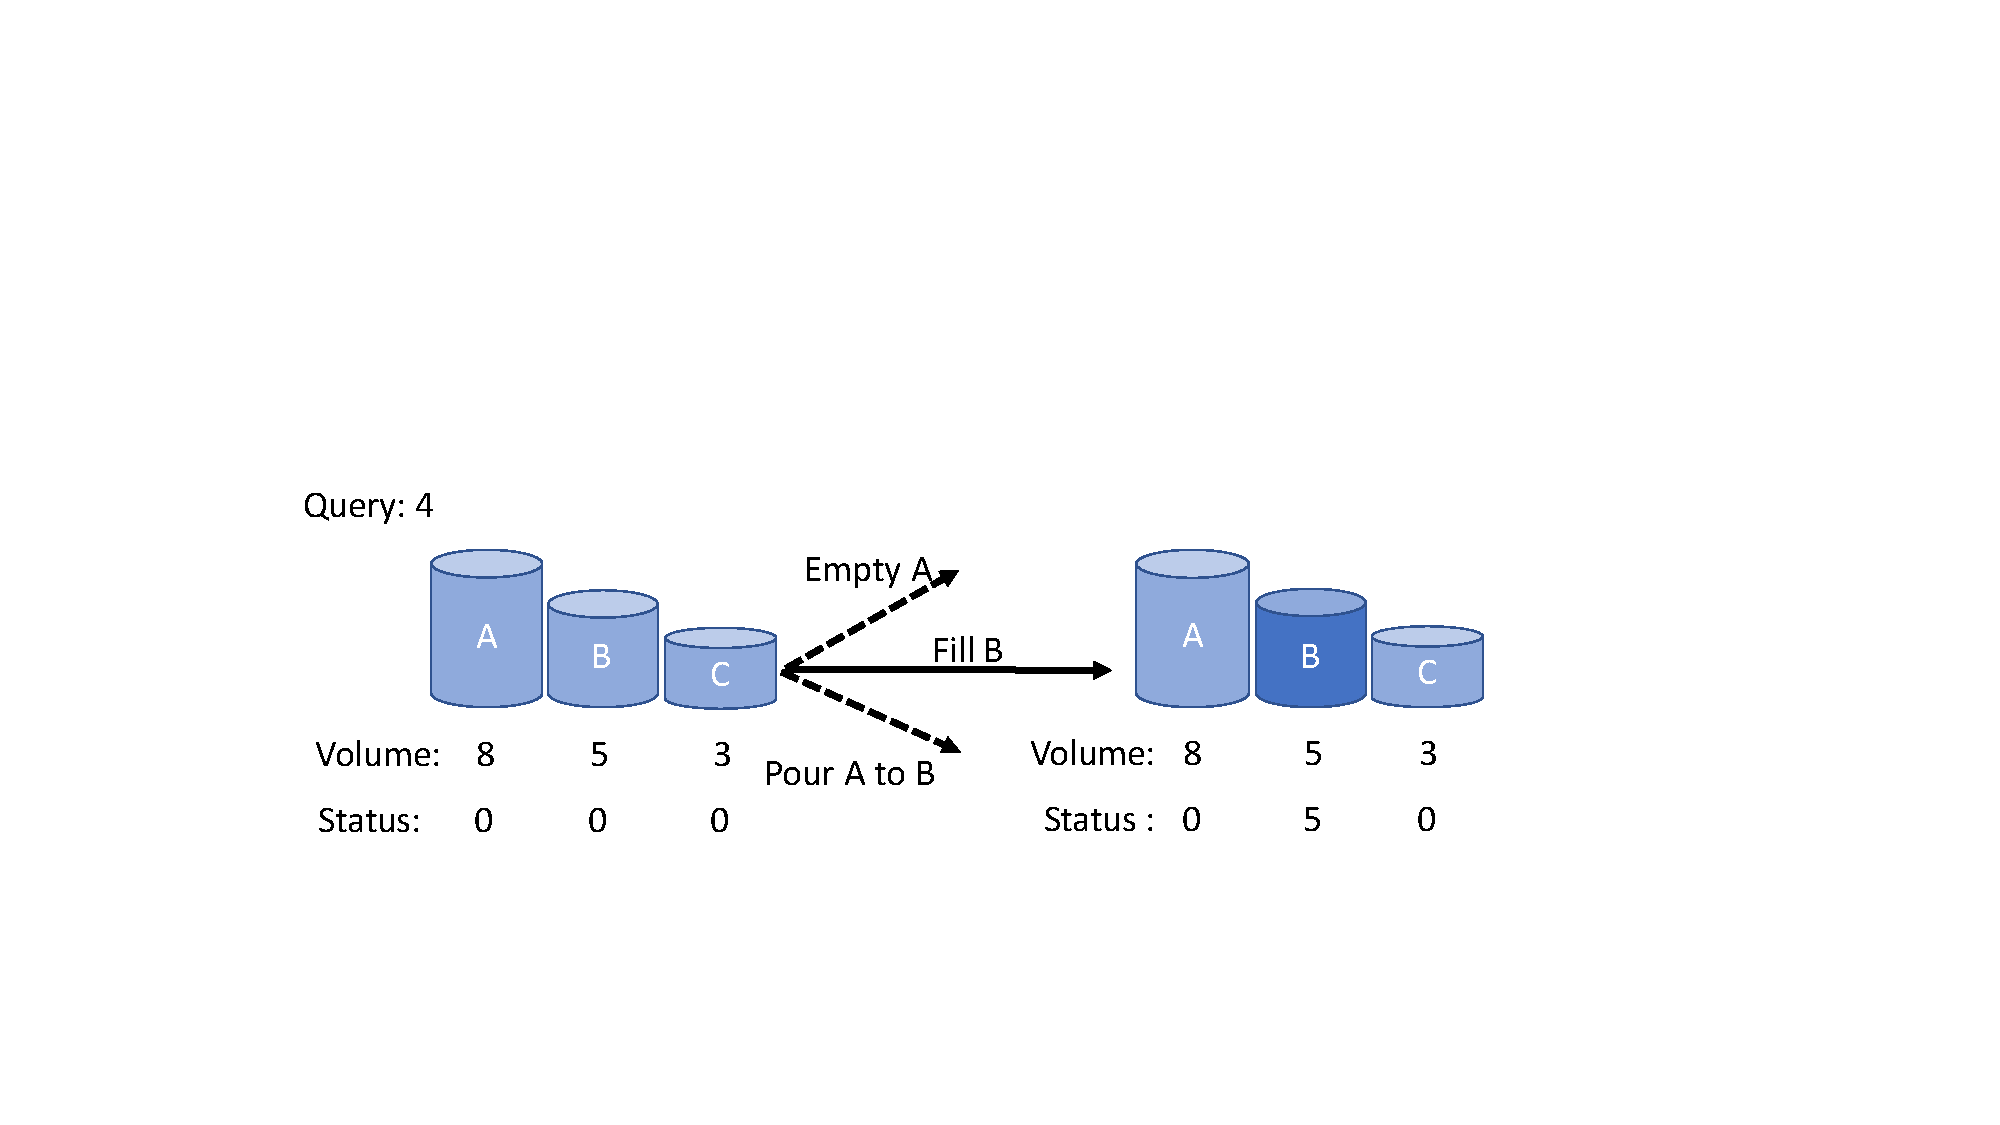
\includegraphics[width=0.5\textwidth]{figures/three_glasses_example_new}
		\caption{Graph traversal in the Three Glass Puzzle problem.}
		\label{fig:reorder_a}
	\end{figure}

\paragraph{An example} Figure \ref{fig:reorder_a} illustrates one step in solving a Three Glass Puzzle. 
	The following action sequences provide one solution to achieve the target $q=4$, given initially empty containers with capacities  $(A=8, B=5, C=3)$, where $a, b, c$ denote the current contents of the containers:
	\begin{itemize}
		\item  {Initial state} $\rightarrow (a=0, b=0, c=0)$  
		\item  {Fill $\mathcal{B}$} $\rightarrow (a=0, b=5, c=0)$ 
		\item  {Pour from $\mathcal{B}$ to $\mathcal{C}$} $\rightarrow (a=0, b=2, c=3)$ 
		\item  {Empty $\mathcal{C}$} $\rightarrow (a=0, b=2, c=0)$ 
    	\item  {Pour from $\mathcal{B}$ to $\mathcal{C}$} $\rightarrow (a=0, b=0, c=2)$ 
		\item  {Fill $\mathcal{B}$} $\rightarrow (a=0, b=5, c=2)$ 
		\item  {Pour from $\mathcal{B}$ to $\mathcal{C}$} $\rightarrow (a=0, b=4, c=3)$
	\end{itemize}
% 	\begin{align}
% 	 \text{initial state} \rightarrow (a=0, b=0, c=0) \\
% 	 \text{fill third container} \rightarrow (a=0, b=0, c=43) \\
% 	 \text{fill second container} \rightarrow (a=0, b=33, c=43) \\
% 	 \text{from second to first } \rightarrow (a=16, b=17, c=43) \\
% 	 \text{empty first container} \rightarrow (a=0, b=17, c=43) \\
% 	 \text{from third to first} \rightarrow (a=16, b=17, c=27) \\
% 	 \text{empty first container} \rightarrow (a=0, b=17, c=27) \\
% 	 \text{from third to first} \rightarrow (a=16, b=17, c=11) \\
% 	 \text{from third to second} \rightarrow (a=16, b=28, c=0)
% 	\end{align}

\paragraph{Data generation} In the Three Glass Puzzle experiments, we randomly draw four integers from $[1, 50)$ to represent the capacities $A, B, C$, and the desired volume $q$. 
We further restrict the values so that $A \geq B \geq C$ and $q < A$, to avoid data duplication. We discard puzzles for which there is no solution. Finally, we keep 600 unique puzzles as the experimental dataset, where 500 puzzles are used for training and the other 100 are used to test a model's generalization capability on the unseen test set.

\paragraph{Experiment settings and hyperparameters}
Let $a, b, c$ be the current status of each container, and define the puzzle status at step $t$ as $n_t = [I_A^T, I_B^T, I_C^T, I_a^T, I_b^T, I_c^T]^T$, where $I_{x}$ is the one-hot representation to encode the value of $x$. 
Given that $A, B, C, a, b$ and $c$ are all smaller than $50$ in the experiment, the dimension of $n_t$ is 300. 
The initial query $q$ is obtained by $q = {E_{mb}}[q]$, where ${E_{mb}}$ is a query embedding lookup table and ${E_{mb}}[x]$ indicates the $x$-th column.
The query embedding dimension is set to $64$.
In the Three Glass Puzzle, there are 13 actions in total: fill one container to its capacity, empty one container, pour one container into another container, and a STOP action to terminate the game. 
We set the maximum length of an action sequence (i.e., the search horizon) to be $12$, where only the STOP action can be taken on the final step.
After the STOP action has been taken, the system evaluates the action sequence and assigns a reward $r = 1$ if the final status is a success, otherwise $r = 0$. The $f_{{\theta}_{S}}$ and $f_{{\theta}_{A}}$ functions are modeled by two different DNNs with the same architecture: two fully-connected layers with 32 hidden dimensions and ReLU activation function.
$f_{{\theta}_{v}}$ is two fully-connected layers with 16 hidden dimensions, where the first hidden layer uses a ReLU activation function and the output layer uses a linear activation function. 
$f_{{\theta}_{q}}$ is modeled by a GRU with hidden size 64.
The hyperparameters in PUCT are set to $c=0.5$ and $\beta=0.2$. We use the ADAM optimization algorithm with learning rate $0.0005$ during training, and we set the mini-batch size to $8$.


\begin{table}[t]
	\centering
	{%\small
		\caption{A List of actions for each container in the Three Glass Puzzle. The agent can also determine to take the STOP action to terminate the game.}
		\label{tab:puzzle_actions}
		\begin{tabular}{|c|c|c|c|}
			\hline
			 Empty $\mathcal{A}$ & Fill $\mathcal{A}$ & Pour $\mathcal{A}$ to $\mathcal{B}$  & Pour $\mathcal{A}$ to $\mathcal{C}$ \\
			 \hline
			 Empty $\mathcal{B}$ & Fill $\mathcal{B}$ & Pour $\mathcal{B}$ to $\mathcal{A}$  & Pour $\mathcal{B}$ to $\mathcal{C}$ \\
			 \hline
			 Empty $\mathcal{C}$ & Fill $\mathcal{C}$ & Pour $\mathcal{C}$ to $\mathcal{A}$  & Pour $\mathcal{C}$ to $\mathcal{B}$ \\
			\hline
		\end{tabular}
	}
\end{table}



\label{Appendix:puzzle_details}


\subsubsection{Knowledge Base Completion}
\label{Appendix:kbc_details}

\begin{table}[t]
\caption{Knowledge base completion datasets statistics.}
\label{tab:kbc_stats}
\centering
\begin{tabular}{c cccccc}
\toprule
Dataset  & \# Train & \# Test & \# Relation & \# Entity & avg. degree & median degree\\
\midrule
WN18RR & 86,835 & 3,134 & 11 & 40,943 &  2.19 & 2 \\
NELL-995 & 154,213 & 3,992 & 200 & 75,492 & 4.07 & 1 \\
FB15K-237 & 272,115 & 20,466 & 237 & 14,541 & 19.74 & 14\\
\bottomrule
\end{tabular}
\end{table}

\paragraph{Statistics of the three datasets}
The NELL-995 knowledge dataset contains $75,492$ unique entities and $200$ relations. 
WN18RR contains $93,003$ triples with $40,943$ entities and $11$ relations. And FB15k-237, a subset of FB15k where inverse relations are removed, contains $14,541$ entities and $237$ relations. The detailed statstics are shown in Table \ref{tab:kbc_stats}.
%\COMMENT{FB15k-237, a subset of FB15k where inverse relations are removed, contains $14,541$ entities and $237$ relations.}

\paragraph{Experiment settings and hyperparameters}
For the proposed \modelname, we set the entity embedding dimension to $4$ and relation embedding dimension to $64$.
The maximum length of the graph walking path (i.e., the search horizon) is $8$ in the NELL-995 dataset and $5$ in the WN18RR dataset.
After the STOP action has been taken, the system evaluates the action sequence and assigns a reward $r = 1$ if the agent reaches the target node, otherwise  $r = 0$.
The initial query $q$ is the concatenation of the entity embedding vector and the relation embedding vector. 
The $f_{{\theta}_{S}}$ and $f_{{\theta}_{A}}$ functions are modeled by two different DNNs with the same architecture: two fully-connected layers with 64 hidden dimensions and the ReLU activation function.
$f_{{\theta}_{v}}$ is two fully-connected layers with 16 hidden dimensions, where the first hidden layer uses a Tanh activation function and the output layer uses a linear activation function. 
$f_{{\theta}_{q}}$ is modeled by a GRU with hidden size 64.
The hyperparameters in PUCT are set to $c=2$ and $\beta=0.5$. 
We roll out $32$ MCTS paths in both training and testing in the NELL-995 dataset and $128$ MCTS paths in the WN18RR dataset.
We use the ADAM optimization algorithm for model training with learning rate $0.0001$, and we set the mini-batch size to $8$.



%For knowledge base completion, the relation embedding dimension is 64 and the entity embedding dimension is 4. {\color{blue} @yeshen, setup details, max step etc.}



% ----------------------------------------------------
\section{Additional Experiments}
\label{Appendix:AdditionalExperiments}
\subsection{The Three Glass Puzzle task in different settings}
\label{Appendix:MCTSTesting}


	
	\begin{figure}[t!]
		\centering
		\subfigure[Test Beam / Rollout = 128]{
			%		\label{fig:reorder_a}
			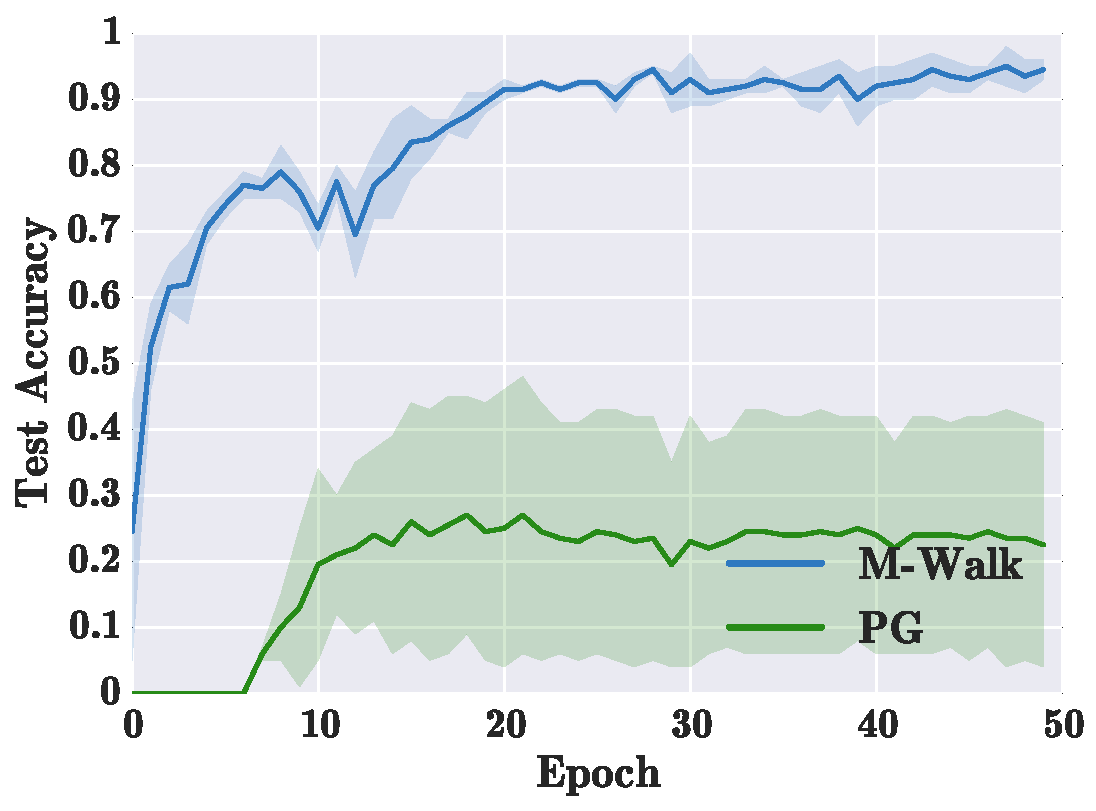
\includegraphics[width=0.28\textwidth]{figures/test_acc_32_128}
		}
		\subfigure[Test Beam / Rollout = 300]{
			%	\label{fig:reorder_a}
			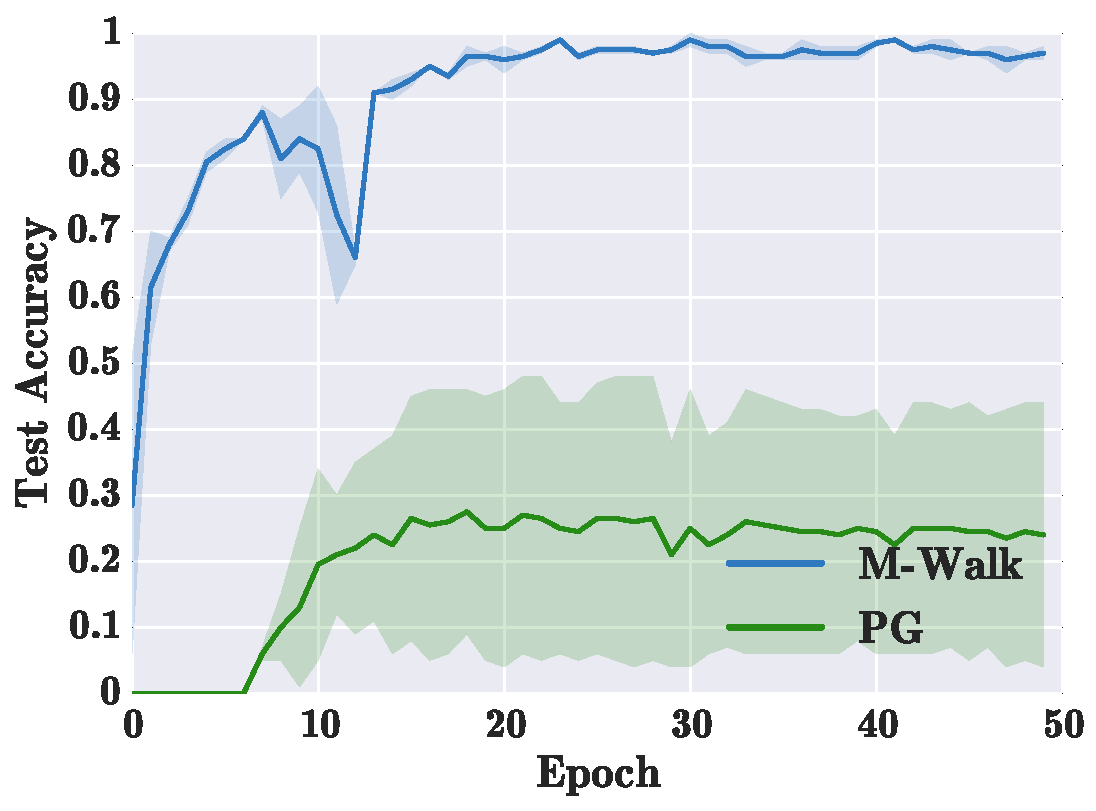
\includegraphics[width=0.28\textwidth]{figures/test_acc_32_300}
		}
		\caption{Three Glass Puzzle test accuracy, where ``PG'' stands for policy gradient.}
		\label{fig:puzzle_test_accuracy}
	\end{figure}

	\begin{table}[t]
		\centering
		\caption{Three Glass Puzzle test accuracy (\%), where ``Beam'' denotes beam search.}
		\label{tab:lp_results}
        \resizebox{\columnwidth}{!}{%
		{%\small
% 			\begin{tabular}{|r|c|c|c|c|}
\begin{tabular}{|l|c|c|c|c|c|c|c|}
\hline
% \cline{2-8}
% & \multicolumn{7}{c|}{Size}                                                                \\ \cline{2-8} 
Size & 1          & 10         & 50         & 100        & 200        & 300        & 400        \\ \hline
\multicolumn{1}{|l|}{PG (Beam)}     & 9.3 (2.1)  & 30.7 (4.5) & 39.3 (3.2) & 45.3 (4.5) & 47.7 (3.2) & 48.7 (3.2) & 49.0 (2.6) \\ \hline
\multicolumn{1}{|l|}{M-Walk (Beam)} & 18.0 (1.7) & 46.0 (7.0) & 60.3 (7.8) & 67.0 (7.0) & 69.0 (6.2) & 69.3 (6.4) & 71.7 (4.5) \\ \hline
\multicolumn{1}{|l|}{M-Walk (MCTS)} & {\bf 18.0} (1.7) & {\bf 63.3} (5.0) & {\bf 84.3} (3.1) & {\bf 90.7} (2.5) & {\bf 95.0} (2.6) & {\bf 96.3} (1.5) & {\bf 99.0} (1.0) \\ \hline
\end{tabular}}
% \multicolumn{1}{l|}{}                          & \multicolumn{4}{c|}{Test Accuracy (\%)}                                                                                                        \\ \hline
% Size & 	 \begin{tabular}[c]{@{}c@{}}PG\\  (Beam)\end{tabular} & \begin{tabular}[c]{@{}c@{}}A2C \\ (Beam)\end{tabular} &\begin{tabular}[c]{@{}c@{}}\modelname\\  (Beam)\end{tabular} & \begin{tabular}[c]{@{}c@{}}\modelname~\\ (MCTS)\end{tabular} \\ \hline
% %		\diagbox[width=10em]{Size}{Model}& 	 \begin{tabular}[c]{@{}c@{}}PG\\  (Beam)\end{tabular} & \begin{tabular}[c]{@{}c@{}}A2C \\ (Beam)\end{tabular} &\begin{tabular}[c]{@{}c@{}}RW\\  (Beam)\end{tabular} & \begin{tabular}[c]{@{}c@{}}RW \\ (MCTS)\end{tabular} \\ \hline
% \multicolumn{1}{|r|}{1}     & 9.3 $\pm$ 2.1 &  9.7 $\pm$ 4.0  & 18.0 $\pm$ 1.7  & 18.0 $\pm$ 1.7  \\ \hline
% \multicolumn{1}{|r|}{10}    & 30.7 $\pm$ 4.5 & 22.3 $\pm$ 1.5 & 46.0 $\pm$ 7.0  & 63.3 $\pm$ 5.0  \\ \hline
% \multicolumn{1}{|r|}{50}    & 39.3 $\pm$ 3.2 & 34.3 $\pm$ 3.1 & 60.3 $\pm$ 7.8  & 84.3 $\pm$ 3.1  \\ \hline
% \multicolumn{1}{|r|}{100}   & 45.3 $\pm$ 4.5 & 39.3 $\pm$ 2.3 & 67.0 $\pm$ 7.0  & 90.7 $\pm$ 2.5  \\ \hline
% \multicolumn{1}{|r|}{200}   & 47.7 $\pm$ 3.2 & 46.3 $\pm$ 3.2 & 69.0 $\pm$ 6.2 &  95.0 $\pm$ 2.6  \\ \hline
% \multicolumn{1}{|r|}{300}   & 48.7 $\pm$ 3.2 & 46.0 $\pm$ 1.0 & 69.3 $\pm$ 6.4 &  96.3 $\pm$ 1.5  \\ \hline
% \multicolumn{1}{|r|}{400}   & 49.0 $\pm$ 2.6 & 46.3 $\pm$ 1.5 & 71.7 $\pm$ 4.5  & 99.0 $\pm$ 1.0  \\ \hline
% 			\end{tabular}
		}
	\end{table}
	
		\begin{table}[t]
		\centering
		{%\small
			\caption{BFS, DFS and \modelname~on Three Glass Puzzle.}
			\label{tab:graph_traversal_results}
			\begin{tabular}{|c|c|c|}
				\hline
				{Method} & {Average \# Steps} & {Max \# Steps} \\
				\hline
				BFS & 264.7 & 1030 \\
				DFS & 192.2 & 1453 \\
				\modelname~& 94.9 & 897 \\
				\hline
			\end{tabular}
		}
	\end{table}
	
We now present more experiments on the Three Glass Puzzle task under different settings. First, to see how fast \modelname~converges, we show in Figure \ref{fig:puzzle_test_accuracy} the learning curves of \modelname~and PG. It shows that \modelname~converges much faster than PG and achieves better results on this task. In Table \ref{tab:lp_results}, we report the test accuracy of \modelname~and vanilla policy gradient (REINFORCE/PG) with different beam search sizes and different MCTS rollouts during testing. The number of MCTS simulations for training \modelname~is fixed to be $32$. 
We observe that \modelname~with MCTS achieves the best test accuracy overall. In addition, with larger beam search sizes and MCTS rollouts, the test accuracy improves substantially. Furthermore, replacing the MCTS in \modelname~by beam search at test time degrades the performance greatly, which shows that MCTS is also very important for \modelname~at test time. 

As mentioned earlier, conventional graph traversal algorithms such as Breadth-First Search (BFS) and Depth-First Search (DFS) cannot be applied to the graph walking problem, because the ground truth target node is not known at test time. However, to understand how quickly \modelname~with MCTS can find the correct target node, we compare it with BFS and DFS in the following cheating setup. Specifically, we apply BFS and DFS to the test set of the Three Glass Puzzle task by disclosing the target node to them. In Table \ref{tab:graph_traversal_results}, we report the average traversal steps and maximum steps to reach the target node. The \modelname~with MCTS algorithm is able to find the target node more efficiently than BFS or DFS.
	
	
	
	
	
	
	
	
\subsubsection{Knowledge Graph Link Prediction}
\label{Appendix:kbc}



\begin{figure}[t!]
		\centering
			\subfigure[\scriptsize TeamPlaySports]{
				%		\label{fig:reorder_a}
				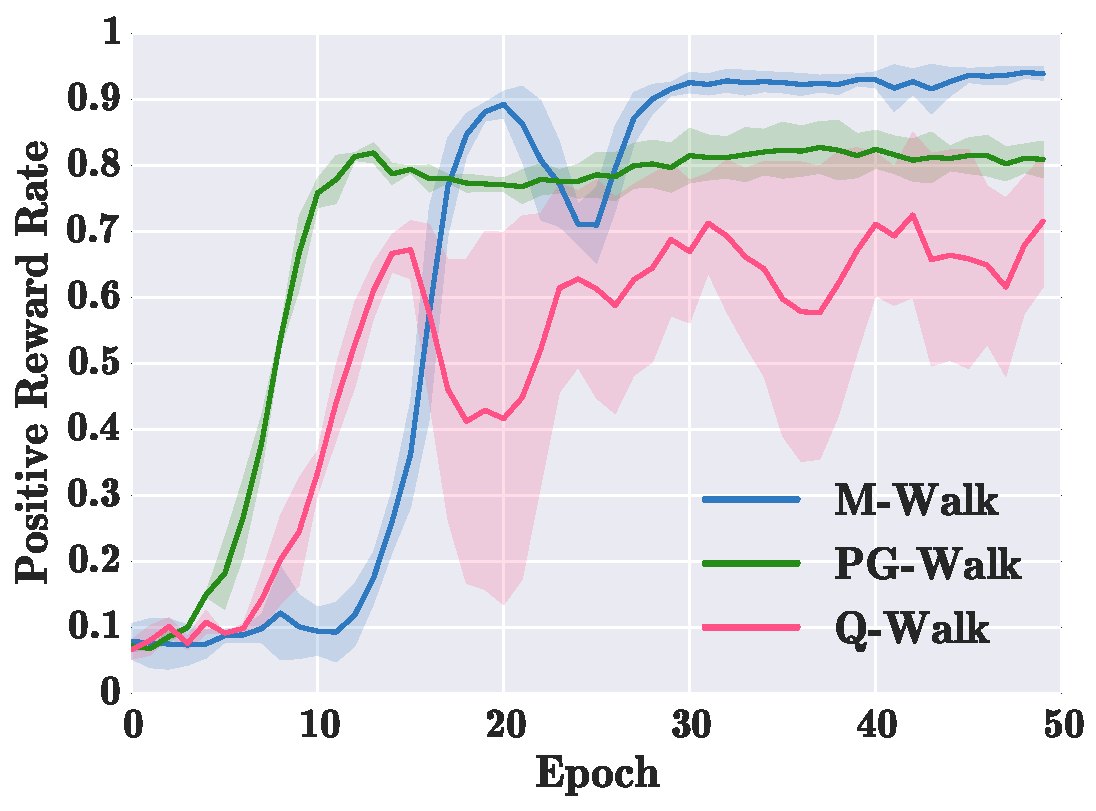
\includegraphics[width=0.31\textwidth]{figures/teamplayssport_success}
			}%\vspace{-2mm}
% 		\subfigure[AthletePlaysForTeam]{
% 			%		\label{fig:reorder_a}
% 			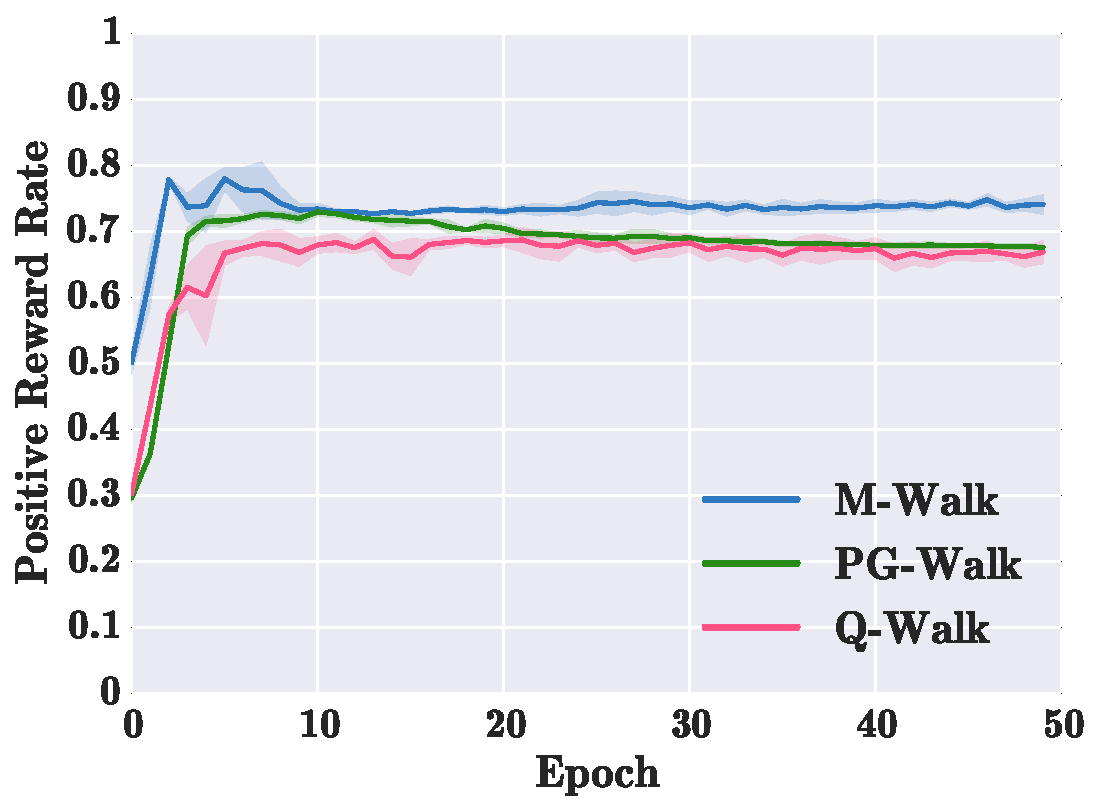
\includegraphics[width=0.31\textwidth]{figures/athleteplaysforteam_success}
% 		}
			\subfigure[\scriptsize AthletePlaysInLeague]{
				%		\label{fig:reorder_a}
				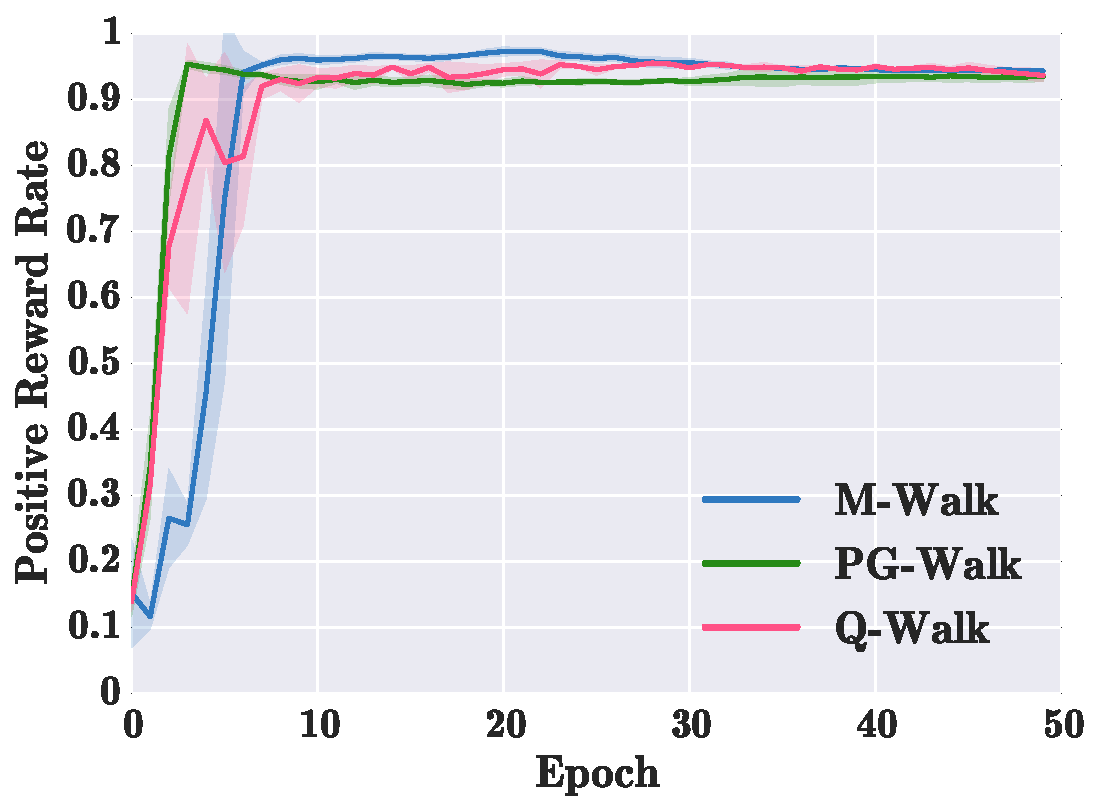
\includegraphics[width=0.31\textwidth]{figures/athleteplaysinleague_success}
			}%
		\subfigure[{\scriptsize AthletePlaysSport}]{
			%	\label{fig:reorder_a}
			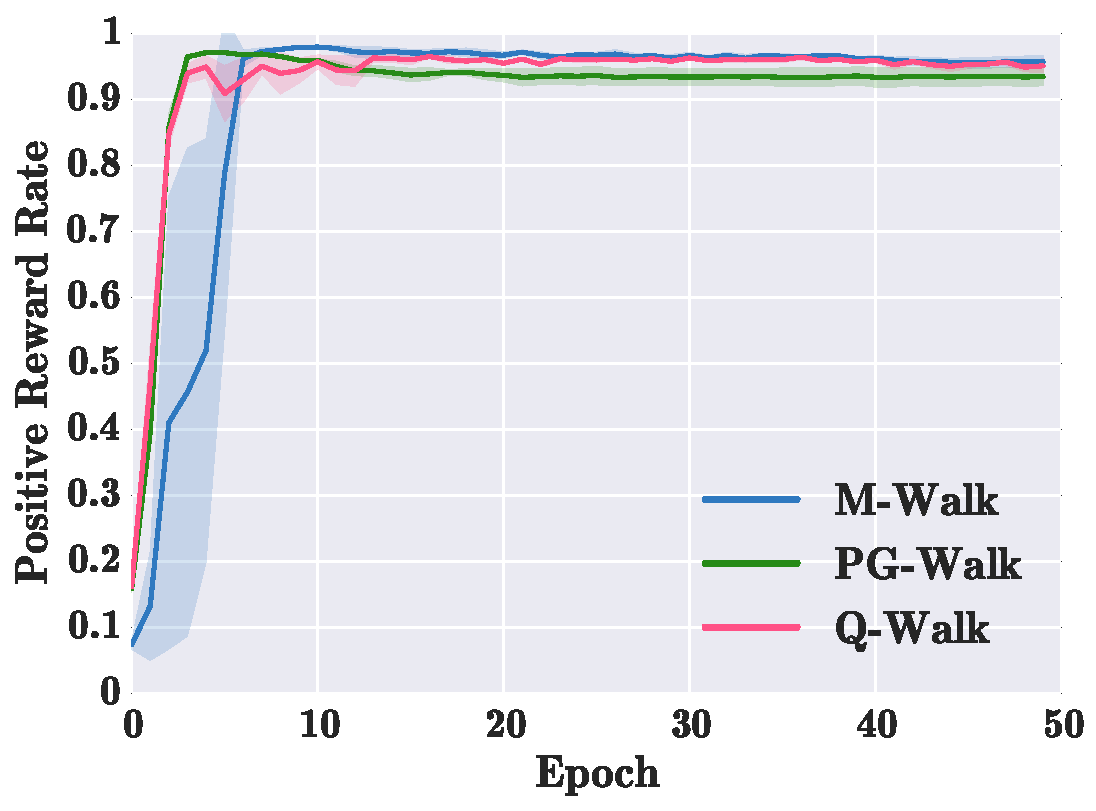
\includegraphics[width=0.31\textwidth]{figures/athleteplayssport_success}
		} %\vspace{-2mm}
			\subfigure[{\scriptsize OrganizationHeadquarterediInCity}]{
			%		\label{fig:reorder_a}
			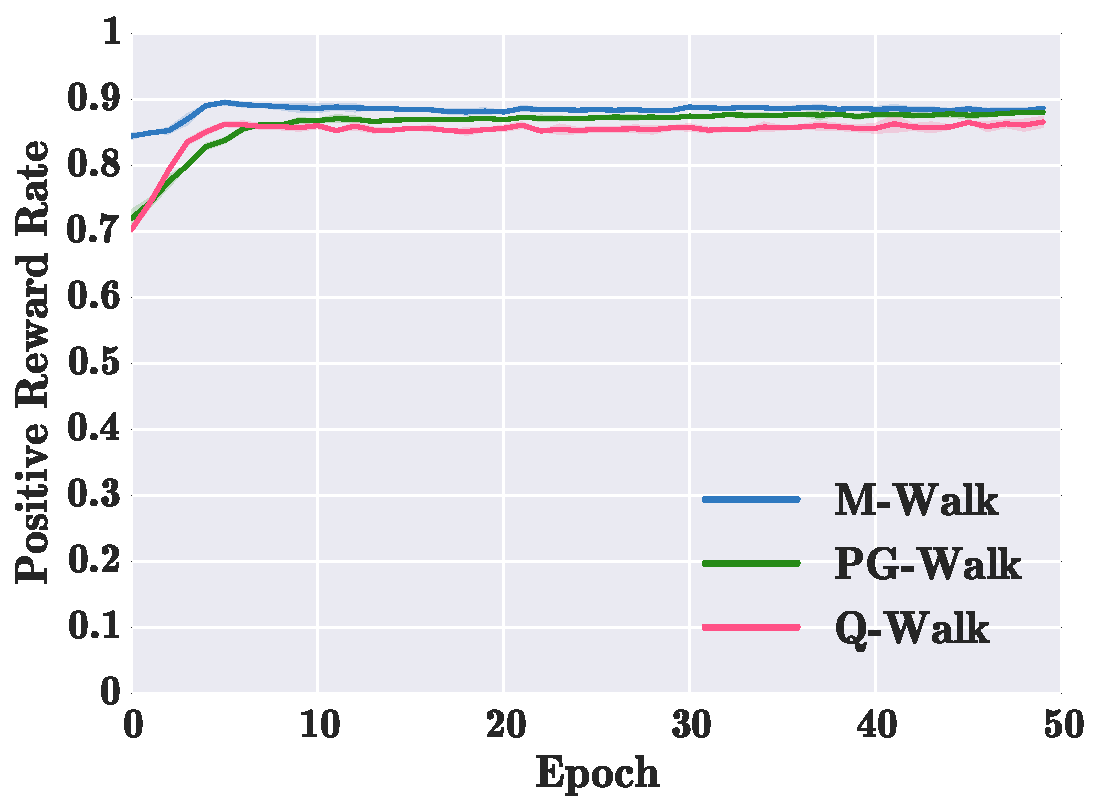
\includegraphics[width=0.31\textwidth]{figures/organizationheadquarteredincity_success}
		}
			\subfigure[\scriptsize PersonBornInLocation]{
			%		\label{fig:reorder_a}
			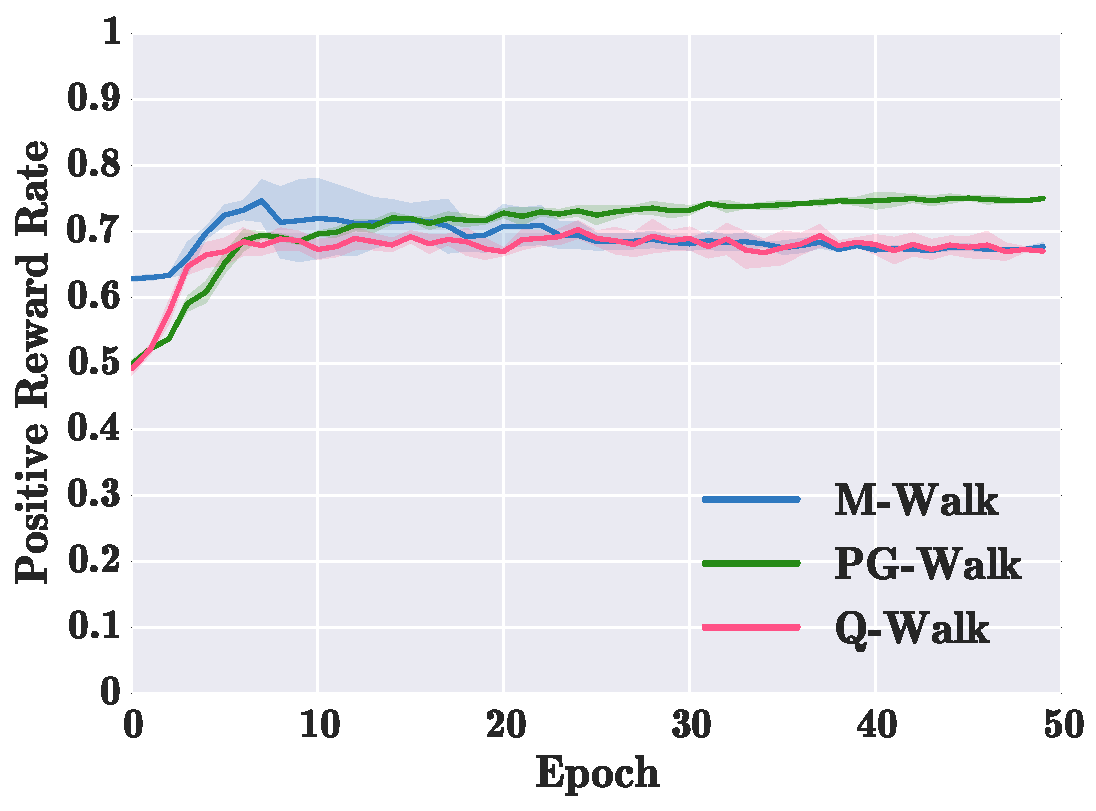
\includegraphics[width=0.31\textwidth]{figures/personborninlocation_success}
		}
			\subfigure[\scriptsize AthleteHomeStadium]{
				%	\label{fig:reorder_a}
				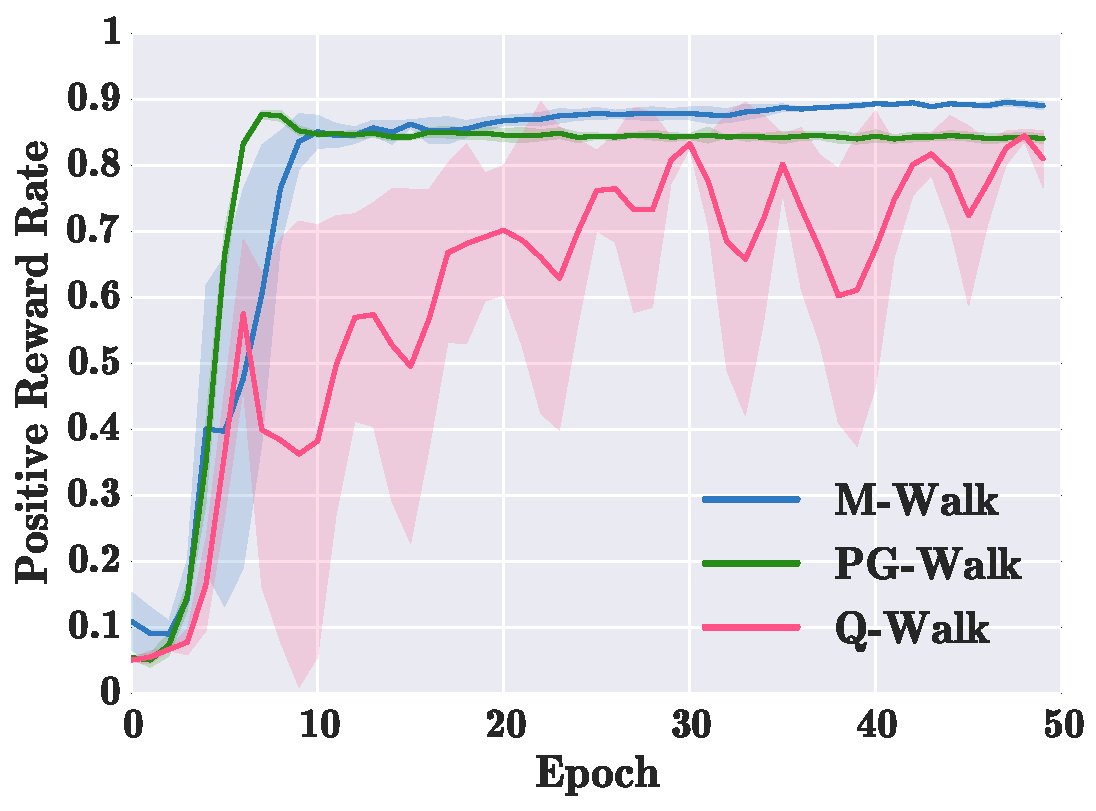
\includegraphics[width=0.31\textwidth]{figures/athletehomestadium_success}
			}%%\vspace{-2mm}
% 			\subfigure[PersonLeadsOrganization]{
% 			%		\label{fig:reorder_a}
% 			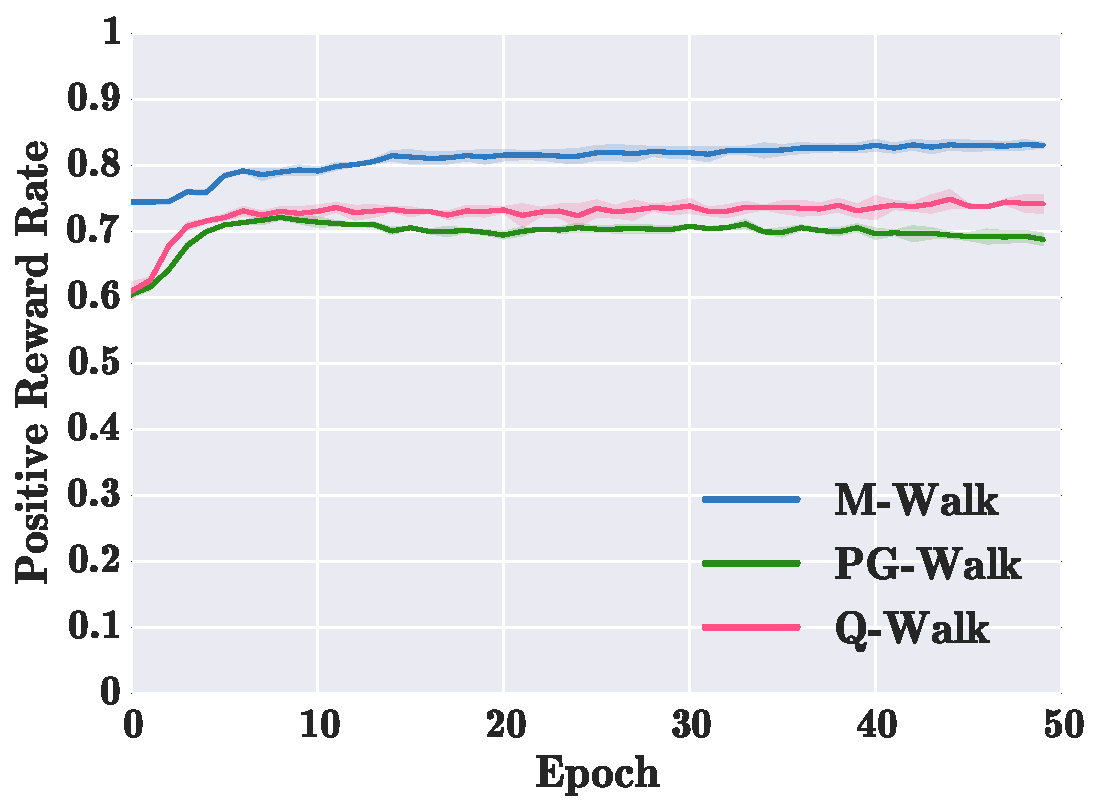
\includegraphics[width=0.31\textwidth]{figures/personleadsorganization_success}
% 		}
%\vspace{-2mm}
		\caption{The positive reward rate during training (i.e., percentage of trajectories with positive reward during training) on the NELL-995 task.}
		\label{fig:kbc_train_success_train2}
	\end{figure}
	
	
	\begin{figure}[t!]
	\centering
	\subfigure[\scriptsize HITS@3]{
		\label{fig:hyperparameter_hit3_analysis}
		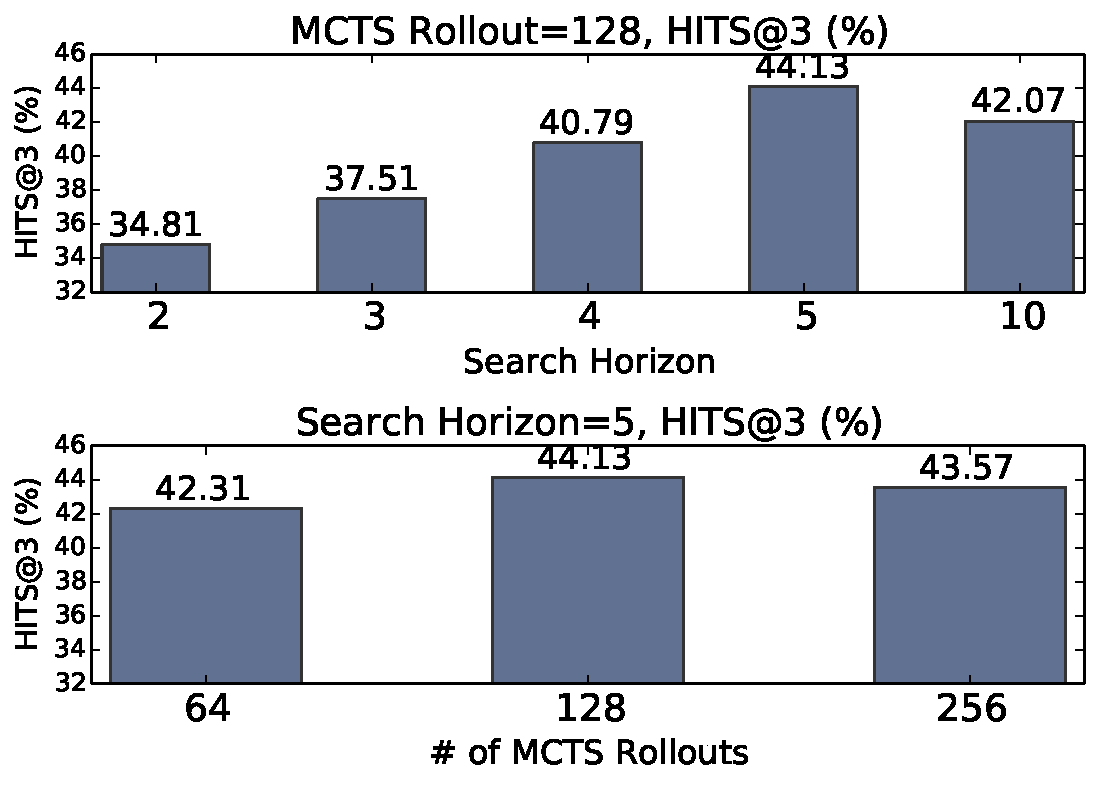
\includegraphics[width=0.31\textwidth]{figures/hyperparameter_HITS_3_analysis.pdf}
	}
	\subfigure[\scriptsize HITS@10]{
		\label{fig:hyperparameter_hit10_analysis}
		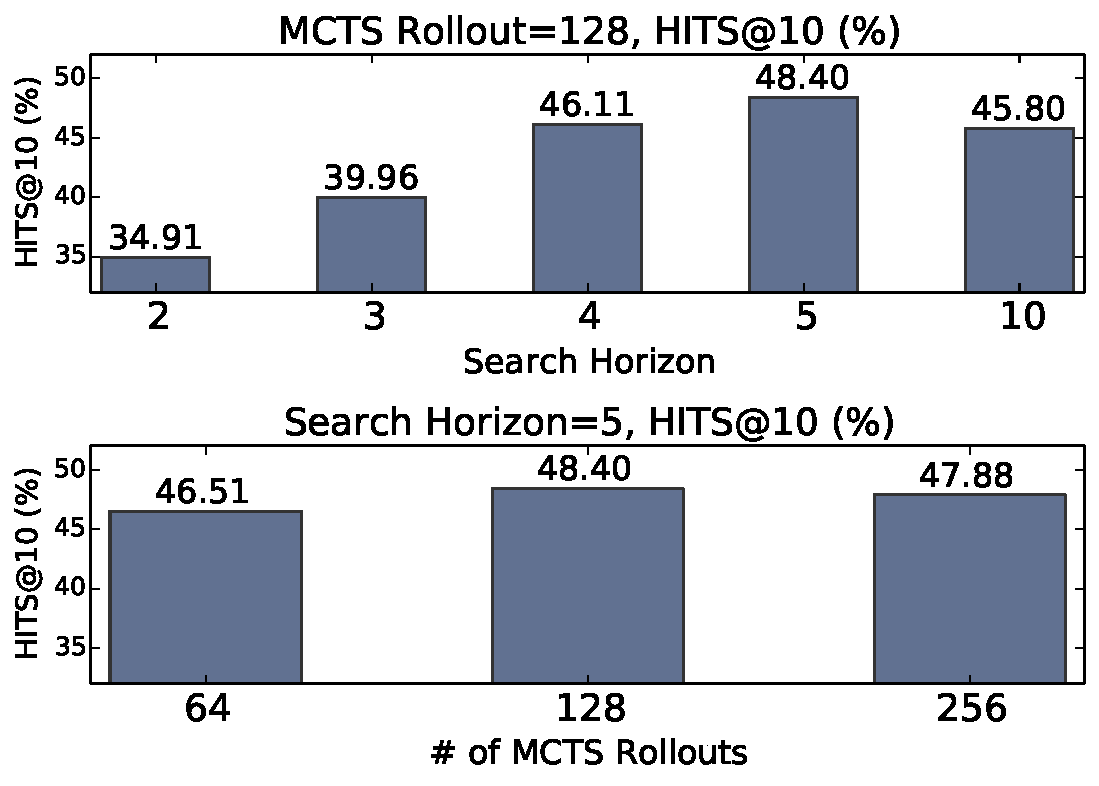
\includegraphics[width=0.31\textwidth]{figures/hyperparameter_HITS_10_analysis}
	}
	\subfigure[\scriptsize Training time]{
		\label{fig:hit1_time}
		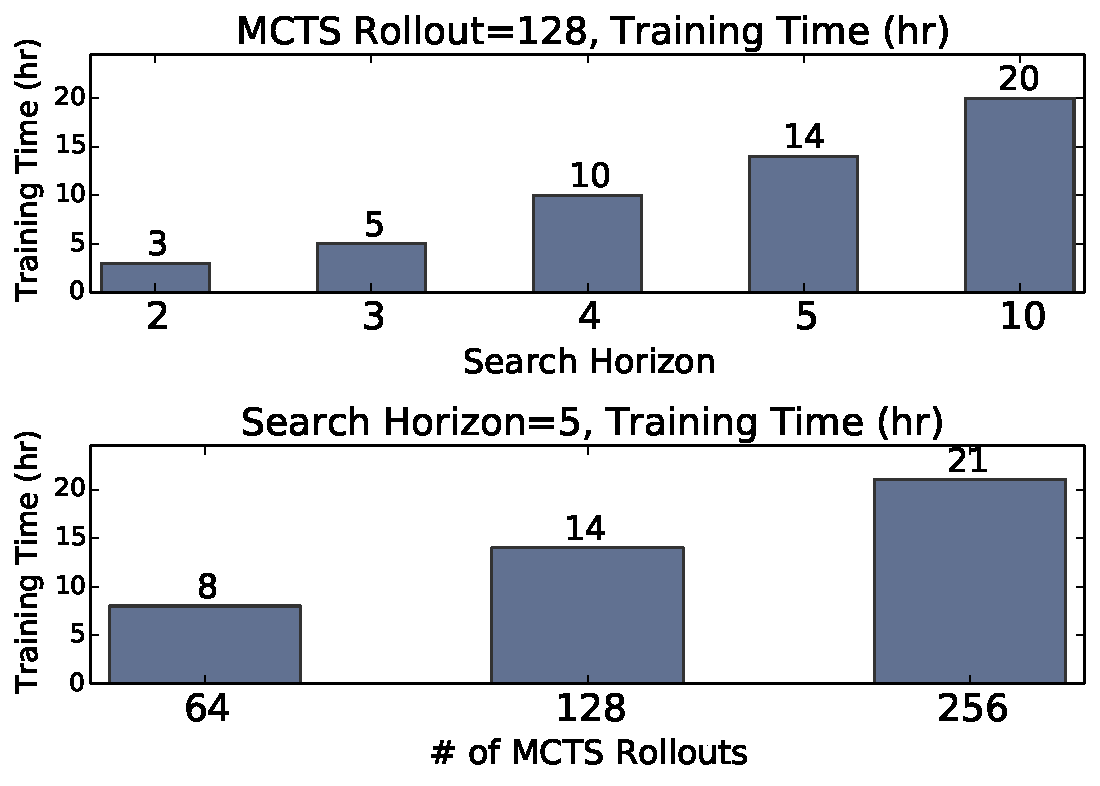
\includegraphics[width=0.31\textwidth]{figures/hyperparameter_TrainingTime_analysis.pdf}
	}%\vspace{-2mm}
	\caption{\modelname~hyperparameter and error analysis on WN18RR.}
	\label{fig:wn18rr_analysis2}
	\end{figure}
	
	\begin{table}[t]
    \begin{center}
    \caption{{The HITS@K and MRR results on the NELL995 dataset.}}
    \label{tab:nell995_hits}
    {\scriptsize
		 \resizebox{.98\columnwidth}{!}{%
    \begin{tabular}{lccc|ccccc}
    \hline
    Metric (\%) & \modelname & \multicolumn{1}{c}{PG-Walk} & \multicolumn{1}{c|}{Q-Walk} & MINERVA    & ComplEx    & \multicolumn{1}{l}{ConvE} & \multicolumn{1}{l}{DistMult}   \\\hline
    HITS@1      & {\bf 68.4}  & 66.7 & 66.8 & 66.3 & 61.2 & 67.2 & 61.0  \\
    HITS@3      & {\bf 81.0}  & 77.5 & 77.3 & 77.3 & 76.1 & 80.8 & 73.3  \\
    MRR         & {\bf 75.4}  & 74.8 & 74.5 & 72.5 & 69.4 & 74.7 & 68.0 \\ \hline
    % \hline
    \end{tabular}}
    }%
    \end{center}
    \end{table}
    
    	
    \begin{table}[ht]
    \begin{center}
    \caption{{The results on the FB15k-237 dataset, in the form of ``mean (standard deviation)''.}}
    \label{tab:fb15k237}
    {\scriptsize
		 \resizebox{.98\columnwidth}{!}{%
    \begin{tabular}{lccc|ccccc}
    \hline
    Metric (\%) & \modelname & \multicolumn{1}{c}{PG-Walk} & \multicolumn{1}{c|}{Q-Walk} & MINERVA    & ComplEx    & \multicolumn{1}{l}{ConvE} & \multicolumn{1}{l}{DistMult} & NeuralLP   \\\hline
    HITS@1      &  16.5(0.3) &  14.8(0.2)   &  15.5(0.2)  & 14.1(0.2) & 20.8(0.2)  & 23.3(0.4) & 20.6(0.4) & 18.2(0.6) \\
    HITS@3      &  24.3(0.2) &  23.3(0.3)   &  23.8(0.4)   & 23.2(0.4) & 32.6(0.5)  & 33.8(0.3) & 31.8(0.2) & 27.2(0.3) \\
    MRR         &  23.2(0.2) &  21.3(0.1)   &  21.8(0.2)  & 20.5(0.3) & 29.6(0.2)  & 30.8(0.2) & 29.0(0.2) & 24.9(0.2) \\ \hline
    \end{tabular}}
    }%
    \end{center}
    \end{table}
	
In this section, we first provide additional experimental results for the NELL995 and WN18RR tasks to support our analysis. In Figure \ref{fig:kbc_train_success_train2}, we show the positive reward rate during training on the NELL995 task. And in Figure \ref{fig:wn18rr_analysis2}, we provide more hyperparameter analysis (search horizon and MCTS simulation number) and training-time analysis. Furthermore, in Table \ref{tab:nell995_hits}, we show the HITS@K and MRR results on NELL995.
	
In addition, we conduct further experiments on the FB15k-237 dataset \cite{Kristinafb15k237}, which is a subset of FB15k \cite{bordes2013translating} with inverse relations being removed. We use the same data split and preprocessing protocol as in \cite{dettmers2018conve} for FB15k-237. The results are reported in Table \ref{tab:fb15k237}. We observe that \modelname~outperforms the other RL-based method (MINERVA). However, it is still worse than the embedding-based methods. In future work, we intend to combine the strength of embedding-based methods and our method to further improve the performance of \modelname.
	
	
	
	
\subsection{The Reasoning (Traversal) Paths}
\label{Appendix:three_glass_puzzle_paths}
 %Finally, in Table \ref{tab:kbc_example_paths}, we present several examples of the knowledge graph traversal paths. %Examples of Three Glass Puzzle can be found in Appendix \ref{Appendix:three_glass_puzzle_paths}.
In Table \ref{tab:kbc_example_paths}, we show the reasoning paths of \modelname~on the NELL995 dataset. Each reasoning path is generated by following the edges on the MCTS tree with the highest visiting count $N(s,a)$.


	\begin{table*}[!h]
	\caption{Examples of paths found by \modelname~on the NELL-995 dataset.}
		\centering
% 		\small
 		 \resizebox{\columnwidth}{!}{%
		\begin{tabular}{l l}\hline%\\
		\vspace{1mm}
			(i) \textbf{WorksFor: } %\vspace{1mm}
	        \\% \\
			 \textsf{journalist jerome holtzman} $\xrightarrow{\text{WorksFor}}$? \vspace{-1mm} \\ \\
			 \textsf{journalist jerome holtzman}  $\xrightarrow{\text{JournalistWritesForPublication}}$
			\textsf{website chicago tribune}, (True) 
			\\ \\
			\textsf{politician mufi hannemann} $\xrightarrow{\text{WorksFor}}$? \vspace{-1mm}
			\\ \\
			\textsf{politician mufi hannemann}  $\xrightarrow{\text{PersonHasResidenceInGeopoliticalLocation}}$
			\textsf{city honolulu}, (True) 
			\\ \\
			\textsf{ceo kumar birla} $\xrightarrow{\text{WorksFor}}$? \vspace{-1mm}
            \\ \\
			\textsf{ceo kumar birla}  $\xrightarrow{\text{PersonLeadsOrganization}}$
			\textsf{company hindalco}, (True) 
			\\ \\
			\textsf{professor chad deaton} $\xrightarrow{\text{WorksFor}}$? \vspace{-1mm}
			\\ \\
			\textsf{professor chad deaton}  $\xrightarrow{\text{PersonLeadsOrganization}}$
			\textsf{BiotechCompany baker hughes}, (False) 
			\\ 		
		    \hline\vspace{1mm}
		  %  \\
			(ii) \textbf{TeamPlaySport:}%\vspace{1mm}
			\\ %\\
			\textsf{SportsTeam arizona dismond backs} $\xrightarrow{\text{TeamPlaySport}}$? \vspace{-1mm}
			\\ \\
			\textsf{SportsTeam arizona dismond backs}  $\xrightarrow{\text{TeamHomeStadium}}$
			\textsf{StadiumOrEventVenue chase field} $\xrightarrow{\text{SportUsesStadium}^{-1}}$ \textsf{sport baseball}, (True)
			\\ \\
			\textsf{SportsTeam l\_a kings} $\xrightarrow{\text{TeamPlaySport}}$? \vspace{-1mm}
			\\ \\
			\textsf{SportsTeam l\_a kings}  $\xrightarrow{\text{TeamPlaysAgainstTeam}^{-1}}$
			\textsf{SportsTeam red wings} $\xrightarrow{\text{TeamWonTrophy}}$ \textsf{AwardTrophyTournament stanley cup} $\xrightarrow{\text{ChampionshipGameOfTheNationalSport}}$ \textsf{sport hockey}, (True)
			\\ \\
			\textsf{SportsTeam cleveland browns} $\xrightarrow{\text{TeamPlaySport}}$? \vspace{-1mm}
			\\ \\
			\textsf{SportsTeam cleveland browns}  $\xrightarrow{\text{TeamPlaysAgainsTteam}^{-1}}$
			\textsf{SportsTeam yankees} $\xrightarrow{\text{TeamHomeStadium}}$ \textsf{AwardTrophyTournament yankee stadium} $\xrightarrow{\text{SportUsesStadium}^{-1}}$ \textsf{sport baseball}, (False)
			\\\hline
		\end{tabular}
 		}%
		\label{tab:kbc_example_paths}
	\end{table*}


% Furthermore, in Tables \ref{tab:puzzle_traversal_paths} and \ref{tab:puzzle_traversal_paths2}, we show several traversal paths made by the \modelname~model in the test set of Three Glass Puzzle dataset. 
	

	

	

	


% % 	\begin{table*}
% % 		\centering
% % 		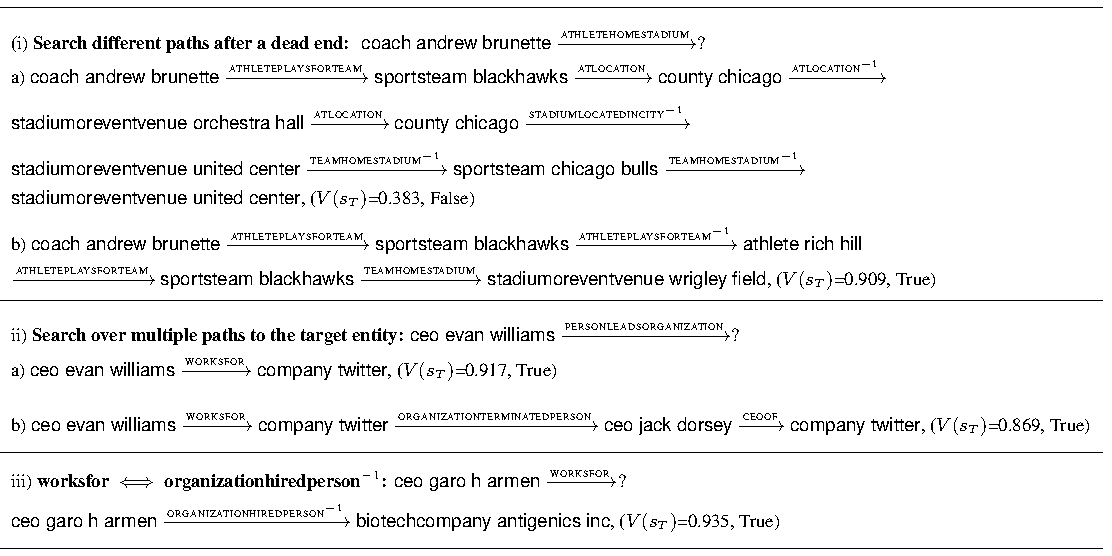
\includegraphics[width=0.8\textwidth]{figures/Table_Path.pdf}
% % 		\caption{Examples of paths found by \modelname~on the NELL-995 dataset. \modelname~can learn to traverse multiple paths to reach the target node (example i) and learn to explore new paths when reach a dead end (example ii).}
% % 		\label{tab:kbc_example_paths}
% % 	\end{table*}
	

	

	
	

% % \subsection{Text Generation}
% % \label{Appendix:TextGeneration}

% % %\paragraph{Text Generation Task.}
% % %For text generation tasks, such as conversation generation \cite{li2016persona} or poem generation \cite{yu2017seqgan}, we can formulate all possible generation space as a graph $\mc{G} = (\mc{N},\mc{E})$  and formulate the problem as a graph walk problem. To be specific, each node $n \in \mc{N}$ represents

% % %we can represents the quantities in the problem as a graph $\mc{G} = (\mc{N},\mc{E})$ and formulate the problem as a graph walk problem. Specifically, each node $n \in \mc{N}$ represents the amounts of liquid remaining in containers $A$, $B$ and $C$, respectively, and each edge represents one of the three feasible actions that could be taken


% % %\subsubsection{Text Generation}
% % %\label{Appendix:text_generation_details}

% % We further evaluate the proposed approach in a text generation task. We can formulate all possible generation space as a graph $\mc{G} = (\mc{N},\mc{E})$ and formulate the text generation task as a graph walk problem.
% % To be specific, each node $n_i \in \mc{N}$ represents a word in the vocabulary and each edge $e_{ij}\in \mc{E}$ represents generating the next word $n_j$ from the current word $n_i$. %{\color{blue} confusing: }Let $q_i$ represent the context embedding of $n_i$.

% % We use the Chinese poem corpus \cite{zhang2014chinese, DBLP:journals/corr/YuZWY16} in the experiments.
% % The corpus consists of $16,394$ Chinese quatrains, each containing four lines with twenty characters in total.
% % We split the dataset into two parts, $90$ percent for training and $10$ percent for testing.
% % We setup the experiments as a conditional generation task.
% % Given the first two lines in a Chinese quatrain, the goal is to generate the following two lines.
% % We use BLEU-2 \cite{Papineni:2002:BMA:1073083.1073135} score as the evaluation metric to measure the similarity between the generated texts and the ground-truth texts.
% % %During testing, the model is given a two lines of Chinese quatrain,
% % %In the testing phase, the model is given with a partial poem, i.e., $(a, b, c, \_\_\_\_)$, and it is asked to generate the rest of it.

% % We build the vocabulary by keeping the most frequent 3,000 words and each word is assigned with a pre-trained 300-dimensional Chinese word embeddings using Chakin.\footnote{https://github.com/chakki-works/chakin} The word embeddings are fixed in our experiments.
% % We use an LSTM language model (denoted as LM) as a baseline. The LM model has three LSTM layer with 300 hidden units in each layer.
% % We implement Self-Critic Sequence Training (SCST) reinforcement learning algorithm \cite{DBLP:journals/corr/RennieMMRG16} as another baseline.
% % The SCST model is initialized by a pretrained LSTM language model and uses BLEU-2 score as reward. 

% % The proposed ReinforceWalk model is also initialized with the pre-trained language model. 
% % We use the the BLEU-2 score as the reward to the ReinforceWalk model. 
% % The ReinforceWalk model performs $64$ rollout for each training instance, where $8$ of them are sampled from the current policy, and the other $56$ rollouts are sampled by the MCTS algorithm.
% % %In the MCTS algorithm, the next word is selected according to both the prior probability (computed by a language model) and statistics in the search tree using a variant of PUCT algorithm \cite{Rosin2011, silver2017mastering}:
% % %	\begin{align}
% % %	w_t &= \nonumber\\
% % %	&\text{argmax}_{w} \left( c_{puct} p(w | s_t)^{\gamma} \frac{\sqrt{\sum_{w'} N(s_t, w')}}{1 + N(s_t, w) } + \frac{R(s_t, w)} {N(s_t, w)}
% % %		 \right)
% % %	\end{align}
% % %where $s_t$ is the LSTM state at time $t$, $N(s_t, w)$ indicates the count of selecting word $w$ at state $s_t$, and $R(s_t, w)$ is the accumulated rewards of selecting $w$ at $s_t$.
% % We set the hyper-parameters $c=0.5$ and $\beta=0.8$ in experiments. The value network $f_{{\theta}_{v}}$ is a three fully-connected layers with 64 hidden units with a Tanh activation function.
% % The $f_{{\theta}_{S}}$ and $f_{{\theta}_{A}}$ functions are identity functions.
% % $f_{{\theta}_{q}}$ is a modeled by a 3-layer LSTM with hidden size 300.
% % In the Table \ref{tab:poem_gen}, we report the evaluation results of the three approaches. 
% % Both LM and SCST baselines use beam search with size 20 during prediction, and RW uses 64 MCTS rollout during prediction. 
% % The proposed model shows significant improvement over baseline LM and SCST models.


% % \begin{table}[h!]
% % 	\centering
% % 	{\small
% % 		\caption{Poem Generation Performance Comparison.}
% % 		\label{tab:poem_gen}
% % 		\begin{tabular}{|c|c|c|c|}
% % 			\hline
% % 			Model & LM & SCST  & RW \\
% % 			\hline
% % 			BLEU-2 (\textperthousand) &  19.35  & 21.83 & {\bf 22.98} \\
% % 			\hline
% % 		\end{tabular}
% % 	}
% % \end{table}





% \begin{table*}[h!]
% 	\centering
% 	{\small
% 		\caption{\modelname~Traversal Paths in Three Glass Puzzle, where ``Index'' stands for MCTS Path Index.}
% 		\label{tab:puzzle_traversal_paths}
% 	 \resizebox{\columnwidth}{!}{%
% 		\begin{tabular}{|c|c|c|c|}
% 			%			\centering
% 			\hline
% 			{Query} & Index & {\modelname~Action Sequence} & Estimated V \\
% 			\hline
% 			\multirow{8}{*}{$(A, B, C, q)$}
% 			& \multirow{3}{*}{0} &
% 			$(0,0,0) \rightarrow (14,0,0) \rightarrow (0,14,0) \rightarrow (14,14,0)  $
% 			& \multirow{3}{*}{1.13e-6} \\
% 			& &
% 			$ \rightarrow (0,14,14) \rightarrow (14,14,14) \rightarrow (0,14,28) \rightarrow (14,14,14)\rightarrow $ & \\
% 			& &
% 			$ (0,14,28) \rightarrow (14,0,28) \rightarrow (14,45,28) \rightarrow (14,26,47) \rightarrow $ END &  \\
% 			\cline{2-4}
% 			\multirow{6}{*}{=(14, 45, 47, 15)}  & \multirow{3}{*}{1} &
% 			$(0,0,0) \rightarrow (0,0,47) \rightarrow (14,0,33) \rightarrow (0,14,33) \rightarrow (14,14,19) $
% 			& \multirow{3}{*}{6.31e-8} \\
% 			& & $ \rightarrow(0,14,19) \rightarrow (14,0,19) \rightarrow (14,19,0)  \rightarrow (14,19,47)  \rightarrow $ & \\
% 			& & $(14,45,21)\rightarrow (14,0,21) \rightarrow (0,14,21) \rightarrow $ END & \\
% 			\cline{2-4}
% 			& ... & ... & ... \\
% 			\cline{2-4}
% 			& \multirow{2}{*}{14} &
% 			$(0,0,0) \rightarrow (0,45,0) \rightarrow (0,0,45) \rightarrow (14,0,31) \rightarrow (14,45,31) \rightarrow$
% 			& \multirow{2}{*}{0.9999} \\
% 			& & $  (14,29,47) \rightarrow (14,29,0) \rightarrow (0,29,14) \rightarrow (14,15,14) \rightarrow $ END & \\
% 			\cline{2-4}
% 			& ... & ... & ... \\
% 			\hline
% 		\end{tabular}
% 		}%
% 	}
% \end{table*}


% \begin{table*}[h!]
% 	\centering
% 	%		\hspace{-250cm}
% 	{\small
% 		\caption{\modelname~Traversal Paths in Three Glass Puzzle, where ``Index'' stands for MCTS Path Index.}
% 		\label{tab:puzzle_traversal_paths2}
% 		 \resizebox{\columnwidth}{!}{%
% 		\begin{tabular}{|c|c|c|c|}
% 			\hline
% 			{Query} & Index & {\modelname~Action Sequence} & Estimated V \\
% 			\hline
% 			\multirow{8}{*}{$(A, B, C, q)$}
% 			& \multirow{3}{*}{0} &
% 			$(0,0,0) \rightarrow (0,0,30) \rightarrow (11,0,30) \rightarrow (0,11,30) \rightarrow (11,11,19) $
% 			& \multirow{3}{*}{2.13e-8} \\
% 			& &
% 			$ \rightarrow (0,11,30) \rightarrow (11,11,19) \rightarrow (0,11,30) \rightarrow (11,0,30)  $ & \\
% 			& &
% 			$\rightarrow (0,11,30) \rightarrow (11,11,30) \rightarrow (7,15,30)  \rightarrow$ END &  \\
% 			\cline{2-4}
% 			\multirow{6}{*}{=(11, 15, 30, 8)}  & \multirow{2}{*}{1} &
% 			$(0,0,0) \rightarrow (0,0,15) \rightarrow (0,0,15) \rightarrow (0,15,15) \rightarrow (11,4,15) $
% 			& \multirow{2}{*}{0.999} \\
% 			& & $ \rightarrow(0,4,26) \rightarrow (4,0,26) \rightarrow (4,15,26)  \rightarrow (11,8,26) \rightarrow $ END & \\
% 			\cline{2-4}
% 			& ... & ... & ... \\
% 			\cline{2-4}
% 			& \multirow{3}{*}{4} &
% 			$(0,0,0) \rightarrow (11,0,0) \rightarrow (0,0,11) \rightarrow (11,0,11) \rightarrow (0,11,11) $
% 			& \multirow{3}{*}{1.72e-8} \\
% 			& & $ \rightarrow(11,11,11) \rightarrow (0,11,22) \rightarrow (11,11,11)  \rightarrow (7,15,11) \rightarrow $  & \\
% 			& & $ (7,0,11) \rightarrow (7,15,11) \rightarrow (7,15,30)  \rightarrow $ END & \\
% 			\cline{2-4}
% 			& ... & ... & ... \\
% 			\hline
% 		\end{tabular}
% 		}%
% 	}
% \end{table*}



